\documentclass[]{iisreport}

\usepackage{pdfpages}

\usepackage{todonotes}

% Uncomment the following line to disable the todo notes.
% \usepackage[disable]{todonotes}

\title{Implementing an OpenMP runtime for MemPool in LLVM}

\author{Diego de los Santos Gausí}
\email{dgausi@student.ethz.ch}

\semester{Spring 2024}
\date{1st of July 2024}
\reporttype{Semester Project}

\professor{Prof.\ Dr.\ L.\ Benini, lbenini@iis.ee.ethz.ch}

\advisor{Samuel Riedel, sriedel@iis.ee.ethz.ch}
\advisor{Sergio Mazzola, smazzola@iis.ee.ethz.ch}

\titlelogo{titlepage_logo}
\titlelogoheight{7cm}

\begin{document}

\frontmatter

\listoftodos

\chapter*{Abstract}

In order to effectively harness MemPool's parallelism, an initial GCC-compatible OpenMP runtime was
developed for this architecture, supporting the most commonly used set of features. However, due to
increasing reliance on the LLVM compiler infrastructure by the MemPool team, it is becoming crucial
to have an OpenMP runtime compatible for it. This project aims to implement an OpenMP runtime that
works with LLVM, supporting at least the same set of features as the previous runtime, while
maintaining comparable performance.

% and offering the possibility of future additions and
%improvements.

% The abstract summarizes what this report is about.
% It focusses on the big picture and does not go into details.
% You should write concisely about the following points:
%
% \begin{itemize}
% 	\item Describe the \textbf{background} of your project: what is the motivation for your project and why is it important?
% 	\item Describe the \textbf{objectives} of your project.
% 	\item Describe the \textbf{problems} that must be addressed to achieve the objectives---why are these problems difficult?
% 	\item Describe your \textbf{approach} and \textbf{methods}.
% 	\item Summarize the most important \textbf{results}.
% 	\item State the main \textbf{conclusion} and its significance.
% \end{itemize}
%
% The abstract typically takes half a page and should not be longer than one full page.
% Try to write a draft of the abstract early on to have a good idea of your project, but revise the abstract as the project progresses.
% Write the final version of the abstract once the report is otherwise complete.
%
% The remainder of this document contains an example on structure and content of the report.
% This template is meant to guide you and not to force you into a certain structure---just make sure you and your advisors agree on content and structure of the report \emph{before} you start writing it.
% \Cref{app:topic-specific_guidelines} gives more specific guidelines for some major project areas (e.g., hardware designs).
% If you are new to \LaTeX{} or want to learn some best practices, you should also check the short \LaTeX{} guide in \cref{app:LaTeX_guide}.

\chapter*{Acknowledgments}

I'd like to sincerely thank Samuel Riedel and Sergio Mazzola for supervising this project. Their
continuous feedback and encouragement has been very helpful, and it enabled me to stay on track and
make steady progress.

I'd also like to thank Frank Gürkaynak for getting me in touch with the group, which led to me
learning about this project.

\chapter*{Declaration of Originality}

Download the official declaration of originality\footnote{\url{https://www.ethz.ch/content/dam/ethz/main/education/rechtliches-abschluesse/leistungskontrollen/declaration-originality.pdf}}, print it, and sign it.
When printing your thesis, replace this sheet with the physically signed original paper.
For the digital version, scan the filled declaration of originality (either before signing or remove your signature\footnote{%
  By removing your signature from the digital version of your report, you enable us to share your report with collaborators without having to deal with privacy concerns.
} from the image) and replace the text inside this file with \verb|\includepdf[scale=0.9]{declaration_of_originality}|.


\tableofcontents

\mainmatter

\chapter{Introduction}
\label{ch:introduction}

Mempool enables parallelism between its up to 256 cores. If one were to
manually manage this parallelism , it would be a tedious and error prone task.
Luckily, there are high level programming abstractions that allow the
programmer to express this parallelism in a clear and concise way. An
example for this is OpenMP~\cite{openmp}.

OpenMP is comprised of a set of compiler directives for both C/C++ and Fortran
that enable this higher level abstraction. In order to use OpenMP, the compiler
has to support it. Support can be roughly divided into two parts:

\begin{enumerate}
	\item The compiler must be able to parse the directives compile the code surrounding them
	      according to their semantics.
	\item The output of the compilation process must match the target platform
	      in order to make use of its parallelism capabilities and primitives.
\end{enumerate}

For that reason, both GCC and LLVM provide an OpenMP runtime library interface that bridges the gap
between both points: instead of directly generating a binary from OpenMP annotated code, the compiler
generates calls to the OpenMP runtime library. This library has to be aware of how to parallelize the
code given the platform, therefore a new runtime library has to be implemented for each target platform.
Naturally, popular compilers ship with their own OpenMP runtime library implementation, however not
targeting embedded systems.

---

The introduction motivates your work and puts it into a bigger context.
It should answer the following questions:
What is the background of this work?
What is the state of the art?
Why is this project necessary to advance the state of the art?
What are the problems that have to be solved and why are they difficult?
What are your contributions to solve these problems?
How do you evaluate your solution to show that it is adequate and applicable?

An introduction written along these questions naturally follows the \textit{\gls{spse}}\footnote{%
	The \acrshort{spse} approach was established in a book~\cite{Hoey83}, but is also briefly summarized in a more recent article~\cite{MP12}, which is available online.
} approach.
In the \emph{situation}, you set the scene for your work and catch the interest of the readers by showing the importance and generality of the scene.
In the \emph{problem}, you spot an issue in the scene and show why and how it significantly taints the scene.
In the \emph{solution}, you outline your solution to that issue.
Finally, in the \emph{evaluation}, you present the main arguments why the claimed solution actually does solve the problem.

In the following chapters, you will elaborate each of the four \gls{spse} elements in detail:
In \textsl{Background}, you lay the foundations for an in-depth understanding of the situation and the problem.
In \textsl{Related Work}, you show how others have address this (or similar) problems and why their solutions are not sufficient or applicable.
In \textsl{Implementation}, you specify your solution, which you then evaluate rigorously for strengths and weaknesses in \textsl{Results}.

At the end of the introduction, you should explicitly show this structure to the reader by briefly explaining how this report is organized.
Instead of using the general \gls{spse} terminology and the chapter names mentioned above, we urge you to use the domain-specific terminology established in the introduction and point to chapters using cross references (e.g., refering to \cref{ch:background} instead of ``the Background chapter'').

\chapter{Background}
\label{ch:background}

Explain the background and theory underlying your project.
Assume that the average reader has the same knowledge you had \emph{before} undergoing this project.
This chapter should transfer all knowledge necessary to understand the following chapters.

As this and the following chapters are likely longer than a few pages, consider structuring them into sections (but avoid fragmentation by overly fine-grained sectioning).
Use the \verb|\..section{}| command family as illustrated below:

\section{First section}
\label{sec:background_overview}

\subsection{First subsection}

\subsection{Second subsection}

\subsubsection{First subsubsection}

Follow a top-down approach when structuring the chapter, and guide the reader by giving a short overview at the beginning of each section.
Again, you can use labels and references (e.g., referring to \cref{sec:background_overview}).

\chapter{Related Work}
\label{ch:related_work}

\section{GCC Implementation}
\label{sec:gcc_implementation}

As previously mentioned, MemPool already had a working OpenMP runtime library for \gls{gcc}. In the
following, we will briefly discuss its architecture and implementation.

\subsection{Event Loop}
\label{subsec:event_loop}

Because the entry point of the application is the same for all cores, it is necessary to distinguish
between master and worker cores at runtime. Therefore, every application intended to use the
\gls{gcc} OpenMP runtime has to include the code shown on \cref{lst:event_loop} in its main file.
Essentially, it distinguishes between two cases:

\begin{enumerate}
	\item If the current core has ID 0 (i.e., it is the master core), it will continue executing
	      standard OpenMP code (i.e., containing \texttt{\#pragma omp parallel} directives, etc.).
	\item Otherwise, it will enter an infinite loop, where the core first goes to sleep and waits
	      for an interrupt, and then participates in the parallel execution of the program by
	      running its assigned task. Waking up other cores and assigning tasks is done by the
	      master core when it encounters OpenMP constructs that require it.
\end{enumerate}

\begin{lstlisting}[language=C, caption={Main Event Loop}, label={lst:event_loop}]
uint32_t core_id = mempool_get_core_id();

if (core_id == 0) {
  /* OpenMP Code */
} else {
  while (1) {
    mempool_wfi();
    run_task(core_id);
  }
}
\end{lstlisting}

\begin{lstlisting}[language=C, caption={run\_task Implementation}, label={lst:run-task},
                   escapechar=@]
typedef struct {
  void (*fn)(void *);
  void *data;
  uint32_t nthreads;
  uint32_t barrier;
  uint8_t thread_pool[NUM_CORES];
} event_t;

void run_task(uint32_t core_id) {
  if (event.thread_pool[core_id]) { @\label{line:run-task-check}@
    event.fn(event.data);
    __atomic_add_fetch(&event.barrier, -1, __ATOMIC_SEQ_CST);
  }
}
\end{lstlisting}

\cref{lst:run-task} shows the implementation of \texttt{run\_task} as well as \texttt{event\_t}.
Since this implementation assumes at most a single team (i.e., group of threads) working on a single
task, it uses a global variable \texttt{event} of type \texttt{event\_t} to store the task
information.

The thread first checks if it is supposed to participate in the parallel execution by checking
whether \texttt{event.thread\_pool[core\_id]} is set. If it is, it executes the function pointed to
by \texttt{event.fn} and decrements the barrier, which makes sure that all threads have finished
their work before starting the next task.

\begin{lstlisting}[language=C, caption={set\_event Implementation}, label={lst:set-event}]
void set_event(void (*fn)(void *), void *data, uint32_t nthreads) {
  uint32_t num_cores = mempool_get_core_count();
  event.fn = fn;
  event.data = data;
  if (nthreads == 0) {
    event.nthreads = num_cores;
    event.barrier = num_cores;
  } else {
    event.nthreads = nthreads;
    event.barrier = nthreads;
  }

  for (uint32_t i = 0; i < num_cores; i++) {
    event.thread_pool[i] = (i < event.nthreads) ? 1 : 0;
  }
}
\end{lstlisting}

A task is set when the master thread calls \texttt{set\_event} (\cref{lst:set-event}) after
encountering an OpenMP construct that requires it. The function pointer and its arguments are passed
through \texttt{fn} and \texttt{data}, respectively. The number of threads that should participate
in the parallel execution is passed through \texttt{nthreads}. If \texttt{nthreads} is 0, all cores
will execute it. This is controlled by the \texttt{event.thread\_pool} array.

\subsection{Parallel Regions}
\label{subsec:parallel_regions}

OpenMP parallel constructs will be transformed into calls to \texttt{GOMP\_parallel}, which is
responsible for setting the current task, waking up all cores, and waiting for them to finish. Note
that this function is only called by the master thread.

\begin{lstlisting}[language=C, caption={GOMP\_parallel Implementation}, label={lst:gomp-parallel},
                   escapechar=@]
void GOMP_parallel_start(void (*fn)(void *), void *data,
                         unsigned int num_threads) {
  set_event(fn, data, num_threads);
  wake_up_all();
  mempool_wfi();
}

void GOMP_parallel_end(void) {
  uint32_t num_cores = mempool_get_core_count();
  while (event.barrier > 0) {
    mempool_wait(4 * num_cores);
  }
}

void GOMP_parallel(void (*fn)(void *), void *data,
                   unsigned int num_threads,
                   unsigned int flags) {
  uint32_t core_id = mempool_get_core_id();
  gomp_new_work_share(); @\label{line:new-work-share}@
  GOMP_parallel_start(fn, data, num_threads);
  run_task(core_id);
  GOMP_parallel_end();
}
\end{lstlisting}

\subsection{Work Sharing Constructs}
\label{subsec:work_sharing_constructs}

Work sharing constructs (e.g., \texttt{for}, \texttt{sections}, etc.) allow for threads in the
current team to distribute the work to be done in a given parallel region. A global variable of type
\texttt{work\_t} is used for the bookkeeping related to these constructs and is initialized by
calling \texttt{gomp_new\_work\_share} (\cref{lst:gomp-parallel}, \cref{line:new-work-share}).

\begin{lstlisting}[language=C, caption={work_t Struct}, label={lst:work-t}]
typedef struct {
  int end;
  int next;
  int chunk_size;
  int incr;

  omp_lock_t lock;

  // for single construct
  uint32_t checkfirst;
  uint32_t completed;
  void *copyprivate;

  // for critical construct
  omp_lock_t critical_lock;

  // for atomic construct
  omp_lock_t atomic_lock;
} work_t;
\end{lstlisting}

As an example for a work sharing construct, \cref{lst:gomp-loop-dynamic} shows the implementation of
the functions required for a dynamically scheduled for loop construct (i.e., \texttt{\#pragma omp
parallel for schedule(dynamic)}).

\texttt{GOMP_parallel_loop\_dynamic} (\cref{line:gomp-parallel-loop-dynamic}) is very similar to
\texttt{GOMP\_parallel}, but it also initializes the loop bounds and chunk size with
\texttt{gomp\_loop\_init} (\cref{line:gomp-loop-init}).

 Each thread calls \texttt{GOMP\_loop\_dynamic\_start} (\cref{line:gomp-loop-dynamic-start}) once
 and \texttt{GOMP\_loop\_dynamic\_next} (\cref{line:gomp-loop-dynamic-next}) continuously afterwards
 until the loop is finished. The former checks if another thread already initialized the loop bounds
 and chunk size, and initializes them if that is not the case. Then, it atomically increments the
 start of the next chunk for the next thread to use and sets the bounds of the current chunk for the
 current thread. This is done again with every call to \texttt{GOMP\_loop\_dynamic\_next}.

 \pagebreak

\begin{lstlisting}[language=C, caption={GOMP Dynamic For Loop Implementation},
                   label={lst:gomp-loop-dynamic}, escapechar=@]
int GOMP_loop_dynamic_start(int start, int end, int incr, @\label{line:gomp-loop-dynamic-start}@
                            int chunk_size, int *istart,
                            int *iend) {
  int chunk, left;
  int ret = 1;

  if (gomp_work_share_start()) { // work returns locked
    gomp_loop_init(start, end, incr, chunk_size);
  }
  gomp_hal_unlock(&works.lock);

  chunk = chunk_size * incr;

  start = __atomic_fetch_add(&works.next, chunk, __ATOMIC_SEQ_CST);

  if (start >= works.end) {
    ret = 0;
  }

  if (ret) {
    left = works.end - start;

    if (chunk > left) {
      end = works.end;
    } else {
      end = start + chunk;
    }
  }

  *istart = start;
  *iend = end;

  return ret;
}

int GOMP_loop_dynamic_next(int *istart, int *iend) { @\label{line:gomp-loop-dynamic-next}@
  int start, end, chunk, left;

  chunk = works.chunk_size * works.incr;
  start = __atomic_fetch_add(&works.next, chunk, __ATOMIC_SEQ_CST);

  if (start >= works.end) {
    return 0;
  }

  left = works.end - start;

  if (chunk > left) {
    end = works.end;
  } else {
    end = start + chunk;
  }

  *istart = start;
  *iend = end;

  return 1;
}

void GOMP_parallel_loop_dynamic(void (*fn)(void *), void *data, @\label{line:gomp-parallel-loop-dynamic}@
                                unsigned num_threads, long start,
                                long end, long incr, long chunk_size) {
  uint32_t core_id = mempool_get_core_id();

  gomp_new_work_share();
  gomp_loop_init(start, end, incr, chunk_size); @\label{line:gomp-loop-init}@

  GOMP_parallel_start(fn, data, num_threads);
  run_task(core_id);
  GOMP_parallel_end();
}

void GOMP_loop_end() {
  uint32_t core_id = mempool_get_core_id();
  mempool_barrier_gomp(core_id, event.nthreads);
}
\end{lstlisting}

\subsection{Barriers}
\label{subsec:barriers}

To implement barriers, the runtime makes calls to \texttt{mempool\_barrier} as implemented in
MemPool's runtime library. It makes use of MemPool's interrupt capabilities to wake up all cores
when the last core reaches the barrier. Note that cores that are not participating in the parallel
execution will also be woken, up but they will immediately go back to sleep because of the check on
\cref{line:run-task-check} in \cref{lst:run-task}.

\begin{lstlisting}[language=C, caption={mempool\_barrier Implementation}, label={lst:mempool-barrier},
                   escapechar=@]
void mempool_barrier(uint32_t num_cores) {
  // Increment the barrier counter
  if ((num_cores - 1) == __atomic_fetch_add(&barrier, 1,
                                            @@__ATOMIC_RELAXED)) {
    @@__atomic_store_n(&barrier, 0, __ATOMIC_RELAXED);
    @@__sync_synchronize(); // Full memory barrier
    wake_up_all();
  }
  // Some threads have not reached the barrier --> Let's wait
  // Clear the wake-up trigger for the last core reaching the barrier
  // as well
  mempool_wfi();
}
\end{lstlisting}

\section{HERO LLVM Implementation}
\label{subsec:hero_llvm_implementation}

\chapter{Implementation}
\label{ch:implementation}

\section{General Architecture}
\label{sec:general-architecture}

The OpenMP runtime library presented in this report is implemented in C++ and is structured into
the following major components:

\begin{itemize}
	\item KMP entrypoints.
	\item C++ classes for each relevant concept (e.g., threads, teams, barriers, etc.).
	\item Supporting code that bridges the gap between higher level concepts and the underlying
	      MemPool architecture.
\end{itemize}

Each of them will be described in more detail in the following sections.

\section{KMP Entrypoints}
\label{sec:kmp-entrypoints}

The KMP entrypoints are the functions that are called at runtime when running an OpenMP program.
During the compilation process, the compiler converts OpenMP directives into calls to these
functions as defined by the internal \gls{api} between the LLVM compiler and the runtime library. An
LLVM OpenMP runtime reference document is available at~\cite{kmpref}, however it is quite out of date
and not very helpful in documenting the expected behavior of the runtime library. For this reason,
using the source code of the default runtime
library\footnote{\url{https://github.com/llvm/llvm-project/tree/main/openmp}}, as well as smaller
third-party implementations\footnote{\url{https://github.com/parallel-runtimes/lomp}} can be quite
helpful.

In the following, we will go trough each of the implemented entrypoints grouped by the OpenMP
construct or clause that requires them.

\subsection{Parallel Construct}
\label{subsec:parallel-construct}

\subsubsection{\texttt{\_\_kmpc\_fork\_call}}
\label{subsubsec:kmpc-fork-call}

\paragraph{Description} This function is called by the master thread of the current team (the
default team contains all cores and the core with ID 0 runs the master thread). It is responsible
for assigning the appropriate number of threads to the team and waking them up, as well as setting
up the task that they will run.

\paragraph{Arguments}
\begin{itemize}
	\item \texttt{loc}: Pointer to a struct containing information about the source code location
	      of the call.
	\item \texttt{argc}: Number of arguments passed to the microtask function.
	\item \texttt{microtask}: Function pointer to the task to be run by each thread in the team.
	\item \texttt{...}: Variable number of arguments to be passed to the microtask function.
\end{itemize}

\paragraph{Implementation} First, it creates a \texttt{kmp::Task} (\todo{ref}) object with the
microtask, arguments casted to a void pointer array, and the number of such arguments. Then, it
obtains the object representing the current thread using \texttt{kmp::runtime::getCurrentThread()}
(\todo{ref}) and calls the \texttt{forkCall} (\todo{ref}) method on it with the task as an argument.

\begin{lstlisting}[language=C, caption={\_\_kmpc\_fork\_call}, label={lst:fork-call},
                   escapechar=@]
void __kmpc_fork_call(ident_t *loc, kmp_int32 argc,
                      kmpc_micro microtask, ...) {
  va_list args;
  va_start(args, microtask);
  kmp::Task kmpMicrotask(microtask, reinterpret_cast<void **>(args),
                         argc);
  kmp::runtime::getCurrentThread().forkCall(kmpMicrotask);
  va_end(args);
};
\end{lstlisting}

\subsubsection{\texttt{\_\_kmpc\_push\_num\_threads}}

\paragraph{Description} This function is called when using the \texttt{num\_threads} clause in a
parallel construct. It is used to request a specific number of threads to be used in the parallel
section.

\paragraph{Arguments}
\begin{itemize}
	\item \texttt{loc}: Pointer to a struct containing information about the source code location
	      of the call.
	\item \texttt{global\_tid}: Global ID of the calling thread.
	\item \texttt{num\_threads}: Requested number of threads.
\end{itemize}

\paragraph{Implementation} This function essentially just calls the \texttt{requestNumThreads}
method (\todo{ref}) on the object representing the current thread obtained by calling
\texttt{kmp::runtime::getThread} (\todo{ref}) with \texttt{global\_tid}.

\begin{lstlisting}[language=C, caption={\_\_kmpc\_push\_num\_threads}, label={lst:push-num-threads},
                   escapechar=@]
void __kmpc_push_num_threads(ident_t *loc, kmp_int32 global_tid,
                             kmp_int32 num_threads) {
  kmp::runtime::getThread(global_tid).requestNumThreads(num_threads);
};
\end{lstlisting}

\subsection{Work Sharing Constructs}

The following entrypoints are used when running work sharing constructs such as static \texttt{for}
loops or \texttt{sections}. Contrary to GOMP, LLVM uses the same entrypoints for both of them.

\subsubsection{\texttt{\_\_kmpc\_for\_static\_init\_4}}

\paragraph{Description} This function is called by every thread at the beginning of a static work
sharing construct. It is responsible for setting the values of \texttt{plastiter}, \texttt{plower},
\texttt{pupper}, and \texttt{pstride} in order to assign a range of iterations to each thread.
Because this assignment is static, the function only needs to be called once per thread. There is a
variant of this function for handling the case where the loop iteration variable is unsigned. The
semantics and implementation are the same except for the type of \texttt{plower}, \texttt{pupper}
and \texttt{plastiter}, which become unsigned.

\paragraph{Arguments}
\begin{itemize}
	\item \texttt{loc}: Pointer to a struct containing information about the source code location
	      of the call.
	\item \texttt{gtid}: Global ID of the calling thread.
	\item \texttt{schedtype}: Type of scheduling to be used.
	      \footnote{\url{
			      https://github.com/llvm/llvm-project/blob/
			      f28c006a5895fc0e329fe15fead81e37457cb1d1/openmp/runtime/src/kmp.h\#L357}}
	\item \texttt{plastiter}: Pointer to the \emph{last iteration} flag. This is set to 1 if the
	      calling thread is the one to execute the last iteration of the loop.
	\item \texttt{plower}: Pointer to the lower bound of the iteration range for the current thread.
	\item \texttt{pupper}: Pointer to the upper bound of the iteration range for the current thread.
	\item \texttt{pstride}: Pointer to the stride of the iteration range.
	\item \texttt{incr}: Increment amount of the loop iteration variable.
	\item \texttt{chunk}: Chunk size.
\end{itemize}

\paragraph{Implementation} This function just calls the \texttt{forStaticInit} method (\todo{ref})
on the object representing the current team.

\begin{lstlisting}[language=C, caption={\_\_kmpc\_for\_static\_init\_4}, label={lst:for-static-init-4},
                   escapechar=@]
void __kmpc_for_static_init_4(ident_t *loc, kmp_int32 gtid,
                              kmp_int32 schedtype,
                              kmp_int32 *plastiter, kmp_int32 *plower,
                              kmp_int32 *pupper, kmp_int32 *pstride,
                              kmp_int32 incr, kmp_int32 chunk) {
  kmp::runtime::getThread(gtid).getCurrentTeam()->forStaticInit(
      loc, gtid, static_cast<kmp_sched_type>(schedtype), plastiter,
      plower, pupper, pstride, incr, chunk);
};
\end{lstlisting}

\subsubsection{\texttt{\_\_kmpc\_for\_static\_fini}}

\paragraph{Description} This function is called when the static work sharing construct is finished.

\paragraph{Arguments}
\begin{itemize}
	\item \texttt{loc}: Pointer to a struct containing information about the source code location
	      of the call.
	\item \texttt{global\_tid}: Global ID of the calling thread.
\end{itemize}

\paragraph{Implementation} This function is not required for the correct implementation of the our
runtime so it does nothing.\footnote{Because the code generated from the OpenMP directives still
	calls this function, it is necessary to implement it even if it is left empty.}

\begin{lstlisting}[language=C, caption={\_\_kmpc\_for\_static\_fini}, label={lst:for-static-fini},
                   escapechar=@]
void __kmpc_for_static_fini(ident_t *loc, kmp_int32 global_tid){};
\end{lstlisting}

\subsection{Dynamic Loops}

\subsubsection{\texttt{__kmpc_dispatch_init_4}}

\paragraph{Description} This function is called once by each thread before running a dynamic
\texttt{for} loop. It is responsible for storing the loop iteration variables and scheduling type so
that they can be used by future calls to \texttt{__kmpc_dispatch_next_4}
(\cref{subsubsec:kmpc-dispatch-next-4}). Just like for the static loop, there is also a variant of
this function that handles unsigned loop iteration variables.

\paragraph{Arguments}
\begin{itemize}
	\item \texttt{loc}: Pointer to a struct containing information about the source code location
	      of the call.
	\item \texttt{gtid}: Global ID of the calling thread.
	\item \texttt{schedtype}: Type of scheduling to be used.
	      \footnote{\url{
			      https://github.com/llvm/llvm-project/blob/
			      f28c006a5895fc0e329fe15fead81e37457cb1d1/openmp/runtime/src/kmp.h\#L357}}
	\item \texttt{lower}: Lower bound of the iteration range for the current thread.
	\item \texttt{upper}: Upper bound of the iteration range for the current thread.
	\item \texttt{incr}: Increment amount of the loop iteration variable.
	\item \texttt{chunk}: Chunk size.
\end{itemize}

\paragraph{Implementation} This function just calls the \texttt{dispatchInit} method (\todo{ref}) on
the object representing the current team after removing any scheduling modifiers from the schedule
variable using the \texttt{SCHEDULE\_WITHOUT\_MODIFIERS} macro since they are not supported by our
runtime.

\begin{lstlisting}[language=C, caption={__kmpc_dispatch_init_4},
                   label={lst:kmpc-dispatch-init-4}, escapechar=@]
void __kmpc_dispatch_init_4(ident_t *loc, kmp_int32 gtid,
                            kmp_int32 schedtype, kmp_int32 lower,
                            kmp_int32 upper, kmp_int32 incr,
                            kmp_int32 chunk) {
  kmp::runtime::getThread(gtid).getCurrentTeam()->dispatchInit(
    loc, gtid,
    static_cast<kmp_sched_type>(SCHEDULE_WITHOUT_MODIFIERS(schedtype)),
    lower, upper, incr, chunk);
}
\end{lstlisting}

\subsubsection{\texttt{__kmpc_dispatch_next_4}}
\label{subsubsec:kmpc-dispatch-next-4}

\paragraph{Description} This function is called by each thread after calling \texttt{dispatchInit}
and after each iteration of the loop. It is responsible for setting the iteration variables for the
current iteration of the loop that the calling thread should execute as well as updating the loop
information shared across the team so that future calling threads can know what work is left to do.
There is also a variant of this function that handles unsigned loop iteration variables.

\paragraph{Arguments}
\begin{itemize}
	\item \texttt{loc}: Pointer to a struct containing information about the source code location
	      of the call.
	\item \texttt{gtid}: Global ID of the calling thread.
	\item \texttt{plastiter}: Pointer to the \emph{last iteration} flag. This is set to 1 if the
	      calling thread is the one to execute the last iteration of the loop.
	\item \texttt{plower}: Pointer to the lower bound of the iteration range for the current thread.
	\item \texttt{pupper}: Pointer to the upper bound of the iteration range for the current thread.
	\item \texttt{pstride}: Pointer to the stride of the iteration range.
\end{itemize}

\paragraph{Return Value} 1 if there is still work to do for the calling thread, 0 otherwise.

\paragraph{Implementation} This function just calls the \texttt{dispatchNext} method (\todo{ref}) on
the object representing the current team.

\begin{lstlisting}[language=C, caption={__kmpc_dispatch_next_4},
                   label={lst:kmpc-dispatch-next-4}, escapechar=@]
int __kmpc_dispatch_next_4(ident_t *loc, kmp_int32 gtid,
                           kmp_int32 *plastiter, kmp_int32 *plower,
                           kmp_int32 *pupper, kmp_int32 *pstride) {
  return static_cast<int>(
      kmp::runtime::getThread(gtid).getCurrentTeam()->dispatchNext(
          loc, gtid, plastiter, plower, pupper, pstride));
}
\end{lstlisting}

\subsection{Critical Sections}

\subsubsection{\texttt{__kmpc_critical and __kmpc_end_critical}}

\paragraph{Description} These functions are used to implement critical sections.\\
\texttt{\_\_kmpc\_critical} is called before entering a critical section and
\texttt{\_\_kmpc\_end\_critical} is called before leaving it.

\paragraph{Arguments}
\begin{itemize}
	\item \texttt{loc}: Pointer to a struct containing information about the source code location
	      of the call.
	\item \texttt{gtid}: Global ID of the calling thread.
	\item \texttt{crit}: Pointer to a region of memory associated with the critical section. 8
	      $\times$ 32 bits are made available by the compiler at the location pointed to by this
	      argument.
\end{itemize}

\paragraph{Implementation} Both of these functions reinterpret the memory location pointed to by
\texttt{crit} as a \texttt{kmp::Mutex} (\todo{ref}) object and use it to lock and unlock access to
the critical section. We use a static assertion to make sure that the size of the
\texttt{kmp::Mutex} object is smaller than the size of the memory region.

\begin{lstlisting}[language=C, caption={__kmpc_critical and __kmpc_end_critical},
                   label={lst:kmpc-critical}, escapechar=@]
typedef kmp_int32 kmp_critical_name[8];

void __kmpc_critical(ident_t *loc, kmp_int32 gtid,
                     kmp_critical_name *crit) {
  static_assert(sizeof(kmp::Mutex) <= sizeof(kmp_critical_name));

  kmp::Mutex *mutex = reinterpret_cast<kmp::Mutex *>(*crit);
  mutex->lock();
};

void __kmpc_end_critical(ident_t *loc, kmp_int32 gtid,
                         kmp_critical_name *crit) {
		Mutex *mutex = reinterpret_cast<kmp::Mutex *>(*crit);
		mutex->unlock();
};
\end{lstlisting}

\subsection{Master and Single Constructs}

\subsubsection{\texttt{__kmpc_master and __kmpc_single}}

\paragraph{Description} These functions are used to implement master and single constructs
respectively. They are called by every thread before entering a master or single section.
\texttt{\_\_kmpc\_master} needs to make sure that only the master thread of the team executes the
section, while \texttt{\_\_kmpc\_single} needs to make sure that only a single thread executes it,
however, it does not need to be the master thread.

\paragraph{Arguments}
\begin{itemize}
	\item \texttt{loc}: Pointer to a struct containing information about the source code location
	      of the call.
	\item \texttt{gtid}: Global ID of the calling thread.
\end{itemize}

\paragraph{Return Value} 1 if the calling thread should execute the section, 0 otherwise.

\paragraph{Implementation} Both \texttt{\_\_kmpc\_master} and \texttt{\_\_kmpc\_single} are
implemented identically for simplicity, since only letting the master thread execute single sections
will always be correct, as there is only a single master thread per team. It essentially obtains the
thread ID of the calling thread by calling \texttt{getTid()} on the thread object and compares it
against 0, returning 1 if they are equal and 0 otherwise.

\begin{lstlisting}[language=C, caption={__kmpc_master and __kmpc_single},
                   label={lst:kmpc-master}, escapechar=@]
kmp_int32 __kmpc_master(ident_t *loc, kmp_int32 gtid) {
  return static_cast<kmp_int32>(
    kmp::runtime::getThread(gtid).getTid() == 0
  );
};

kmp_int32 __kmpc_single(ident_t *loc, kmp_int32 gtid) {
  return static_cast<kmp_int32>(
    kmp::runtime::getThread(gtid).getTid() == 0
  );
};
\end{lstlisting}

\subsubsection{\texttt{__kmpc_end_master and __kmpc_end_single}}

\paragraph{Description} These functions are called after the execution of a master or single section
respectively by the thread that executed it.

\paragraph{Arguments}
\begin{itemize}
	\item \texttt{loc}: Pointer to a struct containing information about the source code location
	      of the call.
	\item \texttt{gtid}: Global ID of the calling thread.
\end{itemize}

\paragraph{Implementation} These functions are not required for the correct implementation of our
runtime so they do nothing.\footnote{Because the code generated from the OpenMP directives still
	calls these functions, it is necessary to implement them even if they are left empty.}

\begin{lstlisting}[language=C, caption={__kmpc_end_master and __kmpc_end_single},
                   label={lst:kmpc-end-master}, escapechar=@]
void __kmpc_end_master(ident_t *loc, kmp_int32 gtid){};

void __kmpc_end_single(ident_t *loc, kmp_int32 gtid){};
\end{lstlisting}

\subsection{Copyprivate Clause}

\subsubsection{\texttt{\_\_kmpc\_copyprivate}}

\paragraph{Description} This function is used to implement the \texttt{copyprivate} clause
associated with a single section. It is called by every thread that participates in the parallel
section after the single section is executed and it is responsible for broadcasting the private data
of the thread executing the single section to the other threads.

\paragraph{Arguments}
\begin{itemize}
	\item \texttt{loc}: Pointer to a struct containing information about the source code location
	      of the call.
	\item \texttt{gtid}: Global ID of the calling thread.
	\item \texttt{cpy\_size}: Size of the private data to be copied.
	\item \texttt{cpy\_data}: Pointer to the private data to be copied.
	\item \texttt{cpy\_func}: Pointer to a function that copies the private data.
	\item \texttt{didit}: 1 if the calling thread executed the single section, 0 otherwise.
\end{itemize}

\paragraph{Implementation} This function just calls the \texttt{copyPrivate} method (\todo{ref}) on
the object representing the current thread.

\begin{lstlisting}[language=C, caption={__kmpc_copyprivate},
                   label={lst:kmpc-copyprivate}, escapechar=@]
void __kmpc_copyprivate(ident_t *loc, kmp_int32 gtid, size_t cpy_size,
                        void *cpy_data,
                        void (*cpy_func)(void *, void *),
                        kmp_int32 didit) {
  kmp::runtime::getThread(gtid).copyPrivate(loc, gtid, cpy_size,
                                            cpy_data, cpy_func, didit);
};
\end{lstlisting}

\subsection{Reduction Clause}

\subsubsection{\texttt{__kmpc_reduce and __kmpc_reduce_nowait}}

\paragraph{Description} These functions are used to implement the reduction clause. The former
performs a barrier after the reduction, while the latter does not.

\paragraph{Arguments}
\begin{itemize}
	\item \texttt{loc}: Pointer to a struct containing information about the source code location
	      of the call.
	\item \texttt{global_tid}: Global ID of the calling thread.
	\item \texttt{num\_vars}: Number of variables to reduce.
	\item \texttt{reduce\_size}: Size of the data to be reduced (in bytes).
	\item \texttt{reduce\_data}: Pointer to the data to be reduced.
	\item \texttt{reduce\_func}: Pointer to the function that performs the reduction on a pair of
	      elements. The result is made available at the location pointed to by the first argument
	      after calling it.
	\item \texttt{lck}: Pointer to a region of memory associated with the critical section used for
	      the reduction. 8 $\times$ 32 bits are made available by the compiler at the location pointed
	      to by this argument.
\end{itemize}

\paragraph{Return Value} 1 for the master thread, 0 for others. 2 if the reduction should be
performed using build in atomic operations.

\paragraph{Implementation} Both functions are implemented identically since they only differ in the
execution of a barrier, which is differentiated when calling \texttt{\_\_kmpc\_end\_reduce\_nowait}
and \texttt{\_\_kmpc\_end\_reduce} (\cref{subsubsec:kmpc-end-reduce}). They always return 2 in order
to use built-in atomic operations for the reduction.

\begin{lstlisting}[language=C, caption={__kmpc_reduce and __kmpc_reduce_nowait},
                   label={lst:kmpc-reduce}, escapechar=@]
kmp_int32 __kmpc_reduce_nowait(ident_t *loc, kmp_int32 global_tid,
                               kmp_int32 num_vars, size_t reduce_size,
                               void *reduce_data,
                               void (* reduce_func)(void *lhs_data,
                                                    void *rhs_data),
                               kmp_critical_name *lck) {
  return 2; // Atomic reduction
}

kmp_int32 __kmpc_reduce(ident_t *loc, kmp_int32 global_tid,
                        kmp_int32 num_vars, size_t reduce_size,
                        void *reduce_data,
                        void (*reduce_func)(void *lhs_data,
                                            void *rhs_data),
                        kmp_critical_name *lck) {
  return __kmpc_reduce_nowait(loc, global_tid, num_vars, reduce_size,
                              reduce_data, reduce_func, lck);
}
\end{lstlisting}

\subsubsection{\texttt{__kmpc_end_reduce and __kmpc_end_reduce_nowait}}
\label{subsubsec:kmpc-end-reduce}

\paragraph{Description} These functions are called after the reduction is done. The former performs
a barrier, while the latter does not.

\paragraph{Arguments}
\begin{itemize}
	\item \texttt{loc}: Pointer to a struct containing information about the source code location
	      of the call.
	\item \texttt{global_tid}: Global ID of the calling thread.
	\item \texttt{lck}: Pointer to a region of memory associated with the critical section used for
	      the reduction. 8 $\times$ 32 bits are made available by the compiler at the location pointed
	      to by this argument.
\end{itemize}

\paragraph{Implementation} \texttt{\_\_kmpc\_end\_reduce\_nowait} does nothing\footnote{Because the
	code generated from the OpenMP directives still calls this function, it is necessary to implement it
	even if it is left empty.}, while \texttt{\_\_kmpc\_end\_reduce} performs a barrier using
\texttt{\_\_kmpc\_barrier} (\cref{subsubsec:kmpc-barrier}).

\begin{lstlisting}[language=C, caption={__kmpc_end_reduce and __kmpc_end_reduce_nowait},
                   label={lst:kmpc-end-reduce}, escapechar=@]
void __kmpc_end_reduce_nowait(ident_t *loc, kmp_int32 global_tid,
                              kmp_critical_name *lck) {}

void __kmpc_end_reduce(ident_t *loc, kmp_int32 global_tid,
                       kmp_critical_name * lck) {
  return __kmpc_barrier(loc, global_tid);
}
\end{lstlisting}

\subsection{Teams Construct}

\subsubsection{\texttt{__kmpc_fork_teams}}
\label{subsubsec:kmpc-fork-teams}

\paragraph{Description} This function is used to implement the \texttt{teams} construct. It is
responsible for creating a league of teams as described in \cref{sec:openmp}.

\paragraph{Arguments}
\begin{itemize}
	\item \texttt{loc}: Pointer to a struct containing information about the source code location
	      of the call.
	\item \texttt{argc}: Number of arguments passed to the microtask function.
	\item \texttt{microtask}: Function pointer to the task to be run by each thread in the team.
	\item \texttt{...}: Variable number of arguments to be passed to the microtask function.
\end{itemize}

\paragraph{Implementation} This function works very similarly to \texttt{__kmpc_fork_call}
(\cref{subsubsec:kmpc-fork-call}) except that it calls the \texttt{forkTeams} method (\todo{ref})
and that the microtask will only be executed by the master thread of each team.

\begin{lstlisting}[language=C, caption={__kmpc_fork_teams}, label={lst:kmpc-fork-teams}, escapechar=@]
void __kmpc_fork_teams(ident_t *loc, kmp_int32 argc,
                       kmpc_micro microtask, ...) {
  va_list args;
  va_start(args, microtask);
  kmp::Task kmpMicrotask(microtask, reinterpret_cast<void **>(args),
                         argc);
  kmp::runtime::getCurrentThread().forkTeams(kmpMicrotask);
  va_end(args);
}
\end{lstlisting}

\subsubsection{\texttt{__kmpc_push_num_teams}}
\label{subsubsec:kmpc-push-num-teams}

\paragraph{Description} This function is used to implement both the \texttt{num_teams} and
\texttt{thread_limit} clauses of the teams construct. \texttt{num\_teams} requests the number of
teams to create and \texttt{thread\_limit} limits the number of threads in each team.

\paragraph{Arguments}
\begin{itemize}
	\item \texttt{loc}: Pointer to a struct containing information about the source code location
	      of the call.
	\item \texttt{global\_tid}: Global ID of the calling thread.
	\item \texttt{num\_teams}: Requested number of teams.
	\item \texttt{num\_threads}: Requested maximum number of threads per team.
\end{itemize}

\paragraph{Implementation} This function first checks if either \texttt{num\_teams} or
\texttt{num\_threads} are greater than 0 and, if so, it sets the corresponding global variables
(\todo{ref}) accordingly.

\begin{lstlisting}[language=C, caption={__kmpc_push_num_teams}, label={lst:kmpc-push-num-teams}, escapechar=@]
void __kmpc_push_num_teams(ident_t *loc, kmp_int32 global_tid,
                           kmp_int32 num_teams,
                           kmp_int32 num_threads) {
  if (num_teams > 0) {
    kmp::runtime::requestedNumTeams = num_teams;
  }

  if (num_threads > 0) {
    kmp::runtime::requestedThreadLimit = num_threads;
  }
}
\end{lstlisting}

\subsection{Barrier}

\subsubsection{\texttt{__kmpc_barrier}}
\label{subsubsec:kmpc-barrier}

\paragraph{Description} This function is called to execute a barrier.

\paragraph{Arguments}
\begin{itemize}
	\item \texttt{loc}: Pointer to a struct containing information about the source code location
	      of the call.
      \item \texttt{global\_tid}: Global ID of the calling thread.
\end{itemize}

\paragraph{Implementation} This function obtains the barrier object associated with the current team
by calling the \texttt{getBarrier} method (\todo{ref}) and executes it by calling \texttt{wait}.

\begin{lstlisting}[language=C, caption={__kmpc_barrier}, label={lst:kmpc-barrier}, escapechar=@]
void __kmpc_barrier(ident_t *loc, kmp_int32 global_tid) {
  kmp::runtime::getThread(global_tid).getCurrentTeam()
                                        ->getBarrier().wait();
};
\end{lstlisting}

\subsection{Miscellaneous}

\subsubsection{\texttt{__kmpc_global_thread_num}}
\label{subsubsec:kmpc-global-thread-num}

\paragraph{Description} This function is used to obtain the global ID of the calling thread.

\paragraph{Arguments}
\begin{itemize}
	\item \texttt{loc}: Pointer to a struct containing information about the source code location
	      of the call.
\end{itemize}

\paragraph{Return Value} Global ID of the calling thread.

\paragraph{Implementation} This function just returns the value returned by
\texttt{mempool_get_core_id}, which is provided by the MemPool runtime library. It is used to obtain
the current core ID, which is the same as the global thread ID since each thread runs on a single
core with the same ID.

\begin{lstlisting}[language=C, caption={__kmpc_global_thread_num}, label={lst:kmpc-global-thread-num},
                   escapechar=@]
kmp_int32 __kmpc_global_thread_num(ident_t *loc) {
  return static_cast<kmp_int32>(mempool_get_core_id());
};
\end{lstlisting}

\section{C++ Classes}
\label{sec:cpp-classes}

\section{Supporting Code}
\label{sec:supporting-code}

{\color{red}
	This chapter explains your contributions, be it algorithms, architectures, libraries, hardware, or others.
	As usual, follow a top-down approach and break the chapter into meaningful sections.
	It may even be necessary to split the chapter into multiple chapters (e.g., to separate architecture from implementation in a hardware design).

	Derive a structure for this chapter that is meaningful for your report and discuss it with your advisors.
}

\chapter{Results}
\label{ch:results}

\section{Evaluation setup}

\subsection{Testing Framework}
\label{subsec:testing-framework}

\section{Correctness}

\section{Performance}

Compare your results to those achieved by others working on similar problems.
This can be done in a separate section or directly in the sections above.

\section{Current limitations}

It's slow :(

\chapter{Conclusion and Future Work}
\label{ch:conclusion}

Draw your conclusions from the results and summarize your contributions.
Point out aspects that need to be investigated further.

The conclusion can be structured inversely to the introduction:
Summarize how the \emph{evaluation} backs the \emph{solution}, which solves the \emph{problem}.
Describe how your contributions improve the \emph{situation} and what other (potentially newly discovered) problems have to be solved in the future.

Be concise: the conclusion normally fits on a single page and is rarely longer than two pages.


\appendix

\chapter{Topic-Specific Guidelines}
\label{app:topic-specific_guidelines}

\section{IC design (ASIC or FPGA) projects}

    For \gls{ic} design projects, the part of the report where you present your main contributions (the \textsl{Implementation} chapter in this template) usually consists of two chapters: \textsl{Hardware Architecture} and \textsl{Design Implementation}.

  \subsection{Hardware architecture}

    In the Hardware Architecture chapter, you should describe the architecture and decisions that led to it.
    Block diagrams and descriptions of control flow, data flow, and interfaces go there.
    The described architecture can be more general than what you actually implemented, e.g., through parameters.

  \subsection{Design implementation}

    The Design Implementation chapter is about the architecture variant you actually implemented.
    It can be meaningful to merge this chapter with the Results chapter to relate central figures of merit directly to implementation choices and tradeoffs; discuss this with your advisors.

    \subsubsection{Functional verification}

      Describe how you verified the design implementation functionally.
      For example, describe how your testbench interfaced the golden model and your circuit.
      \Cref{fig:functional_verification_tb} illustrates a sample setup.

      \begin{figure}
        \centering
        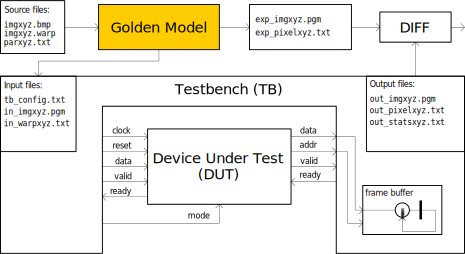
\includegraphics[width=\textwidth]{functional_verification_tb}
        \caption{Testbench used for functional verification.}%
        \label{fig:functional_verification_tb}
      \end{figure}

      Reference a ReadMe file that describes how the testbench can be launched.

    \subsubsection{Back-end implementation}

      In \gls{asic} projects, remember to discuss both front- and back-end implementation.
      That is, if you took special measures for floorplanning, \gls{dft}, or clock or power distribution, you will want to mention it here.
      In this case, make sure to add results that show the impact of your measures.

  \subsection{Results}

    Typical application-specific figures of merit of your hardware design are \gls{snr}, throughput, and memory/interface bandwidth.
    Moreover, you should also specify technology-specific figures such as area (for \glspl{asic}) or resource (for \glspl{fpga}) requirements, timing constraints, and power and energy consumption.

  \subsection{Data sheet}

    If your \gls{asic} is getting fabricated, you need to write a data sheet for it.
    You should put this data sheet into the appendix of your report.
    You are free to write the data sheet in a standalone document and include a \gls{pdf} file here or to write it in the source files of your report.

    Sections of a typical \gls{ic} data sheet are:
    \begin{itemize}
      \item Features
      \item Applications
      \item Packaging
      \item Bonding diagram like the one in \cref{fig:bonding_diagram}.
      \item Pinout diagram like the one in \cref{fig:asic_pinout}.
      \item Interface description
      \item Register map
      \item Operation modes:
      \begin{itemize}
        \item Functional modes
        \item Test modes
      \end{itemize}
      \item Electrical specifications
      \begin{itemize}
        \item Recommended operating regions
        \item Absolute maximum ratings
      \end{itemize}
    \end{itemize}

    \begin{figure}
      \centering
      \includegraphics[width=.75\textwidth]{qfn56_180_std}
      \caption{Standard bonding diagram for QFN56 UMC 180\,nm mini@sics.}%
      \label{fig:bonding_diagram}
    \end{figure}

    \begin{figure}
      \centering
      \includegraphics[width=.75\textwidth]{asic_pinout}
      \caption{Pinout for \textsc{MyFancyChip}.}%
      \label{fig:asic_pinout}
    \end{figure}

    For more information, up-to-date bonding diagrams, and other technology-specific data ask the \gls{dz}.
  % TODO: Remove these two appendices when you no longer need
\chapter{Compact Guide to \LaTeX{} and the \textit{iisreport} Class}
\label{app:LaTeX_guide}

Writing a report with \LaTeX{} might at first not be as intuitive as with \gls{wysiwyg} editors.
However, once you get used to the (rather simple) syntax, you will soon discover how powerful it is and how it helps you achieve tasks that are very difficult (if not impossible) to achieve with \gls{wysiwyg} editors.

This report template provides everything you need to get you started working with \LaTeX{}.
The rest of this chapter contains a short guide with examples for commonly used features.

\section{Building the document}

  Generate a \gls{pdf} file from this template by simply executing \texttt{make} in the directory where the top-level \texttt{.tex} file is in.
  Internally, this will invoke the \texttt{latexmk} program, which is the simplest and most consistent way to build a \LaTeX{} document and is included in all recent \LaTeX{} distributions.
  Additionally, \texttt{make} will check the \texttt{fig/} directory and generate \gls{pdf} files for those figure raw files it knows how to compile (more on this in~\cref{sec:LaTeX_figures}).

\section{Text editing and spacing}

  White spaces and line breaks are automatically inserted when the document is compiled.
  For this, the number of spaces  between  two  words is irrelevant, but a different space length is automatically inserted after a period to make sentences better distinguishable.
  If you write a period that does not end a sentence, e.g., when mentioning Prof.\ Dr.\ S.\ Body, you need to escape the spaces between the abbreviated words with a backslash \verb|\|.
  If you want to prevent \LaTeX{} from breaking a line at a specific white space, you have to replace that space with a tilde \verb|~|.
  \LaTeX{} also automatically hyphenates English words, so it can break a line within a word, although it does so only cautiously.
  Automatic hyphenation can fail, e.g., for non-standard words, causing overly long lines.
  In such cases you have two options:
  First, if you have to break a standard word at an uncommon position, you can insert a \verb|\-| at that position in the word.
  Second, you can define the hyphenation of a non-standard word by adding \verb|\hyphenation{Jab-ber-woc-ky}| to the preamble\footnote{%
    The \emph{preamble} of a document is formed by all code between the \texttt{\textbackslash{}documentclass} command and the beginning of the document body after \texttt{\textbackslash{}begin\{document\}}.
  } of your document.

  A line of text is not broken at the same position as in the source code.
  For this reason, we suggest you put one sentence on one line of source code because this allows your \gls{vcs} to track content changes much better than if you wrap lines within sentences.
  To start a new paragraph, insert an empty line.
  You can manually break a line by writing \verb|\\|; however, this is rarely necessary and wide usage of it is a sign of fighting the typesetting system.

  By default in this template, paragraphs start with a short indentation and are not separated by vertical white space, but this can be changed.
  If you prefer the latter, pass the \texttt{parskip} option to the \texttt{iisreport} document class, i.e., change the first line of your main document to \verb|\documentclass[parskip]{iisreport}|.

  \subsection{Special characters}

    Many special characters are available, and they are all listed in \textsl{The Comprehensive \LaTeX{} Symbol List}~\cite{LaTeXSymbols}.
    At the beginning you might not know what to search for, though, so it can be more helpful to use the \textsl{Detexify}\footnote{\url{http://detexify.kirelabs.org/classify.html}} web app where you can draw the symbol you are looking for.

    A frequent mistake is to mix up the three dashes (-, --, and ---).
    The rules are simple~\cite{Knuth84}:
    \begin{itemize}
      \item The \emph{hyphen}, \verb|-|, is used between the elements of compound words; e.g., ``run-time''.
      \item The \emph{en-dash}, \verb|--|, is used for ranges; e.g., ``3--7''.
      \item The \emph{em-dash}, \verb|---|, is used for digressions within or at the end of a sentence---although you should use it sparingly.
    \end{itemize}

    Another frequent mistake are wrong quotation marks.
    Fortunately, this can also easily be avoided:
    Use \verb|`text'| for `single quotation marks' and \verb|``text''| for ``double quotation marks'' (have a look at the source code to see the matching pairs).
    In American English, double quotes prevail and single quotes are typically only used inside double quotes.

  \subsection{Font faces and emphasis}

    The font face can be changed locally with the commands in \cref{tbl:font_face_commands}.
    The text to appear differently has to be put between the curly braces \verb|{}|, i.e., the text is an \emph{argument} to one of the commands.
    Some font faces can also be combined by nesting them.
    For example, \verb|\textbf{\textit{some words}}| becomes \textbf{\textit{some words}}.

    \begin{table}
      \centerfloat
      \begin{tabular}{ l l }
        \toprule
        \textbf{Command} & \textbf{Output} \\
        \midrule
        \verb|\textrm{}| & \textrm{Roman (the default in this document)} \\
        \verb|\textsf{}| & \textsf{Sans serif} \\
        \verb|\texttt{}| & \texttt{Typewriter (i.e., all characters have the same width)} \\
        \verb|\textbf{}| & \textbf{Bold} \\
        \verb|\textit{}| & \textit{Italic} \\
        \verb|\textsl{}| & \textsl{Slanted} \\
        \verb|\textsc{}| & \textsc{Small caps} \\
        \bottomrule
      \end{tabular}
      \caption{Different font faces.}%
      \label{tbl:font_face_commands}
    \end{table}

    When you want to \emph{emphasize} text, use the \verb|\emph{}| command instead of one of the commands in \cref{tbl:font_face_commands}.
    In this way, you separate a \emph{property} of a piece of text (i.e., which text is emphasized) from its \emph{formatting} (i.e., how emphasized text looks like).
    This is an important principle in typesetting with \LaTeX{}.
    In this case, it allows you to define the formatting of all emphasized text independently of which text is meant to be emphasized.

  \subsection{Font sizes}

    The font size can be changed with the commands in \cref{tbl:font_sizes}.
    These commands change the size within a given \emph{scope}; for instance \verb|{\Large some words}| only prints ``some words'' large.

    \begin{table}
      \newcommand{\sampletext}{quick brown foxes}
      \centerfloat
      \begin{tabular}{ l l }
        \toprule
        \textbf{Command} & \textbf{Output sample} \\
        \midrule
        \verb|\tiny|          & {\tiny \sampletext} \\
        \verb|\scriptsize|    & {\scriptsize \sampletext} \\
        \verb|\footnotesize|  & {\footnotesize \sampletext} \\
        \verb|\small|         & {\small \sampletext} \\
        \verb|\normalsize|    & {\normalsize \sampletext} \\
        \verb|\large|         & {\large \sampletext} \\
        \verb|\Large|         & {\Large \sampletext} \\
        \verb|\LARGE|         & {\LARGE \sampletext} \\
        \verb|\huge|          & {\huge \sampletext} \\
        \verb|\Huge|          & {\Huge \sampletext} \\
        \bottomrule
      \end{tabular}
      \caption{Different font sizes.}%
      \label{tbl:font_sizes}
    \end{table}

  \subsection{Coloring text}

    \begin{figure}
      \centerfloat
      \begin{minipage}{1.1\textwidth}
        % Source: colors from `xcolor`, sorting by own implementation.
        \def\0#1{\colorbox{#1}{\phantom{XX}}~#1\\}
        \scriptsize
        \begin{multicols}{5}
          \noindent
          \0{Magenta}
          \0{Rhodamine}
          \0{VioletRed}
          \0{CarnationPink}
          \0{Lavender}
          \0{RubineRed}
          \0{WildStrawberry}
          \0{OrangeRed}
          \0{Salmon}
          \0{Maroon}
          \0{Red}
          \0{Mahogany}
          \0{BrickRed}
          \0{Melon}
          \0{RedOrange}
          \0{Sepia}
          \0{Brown}
          \0{Bittersweet}
          \0{RawSienna}
          \0{Peach}
          \0{Orange}
          \0{Tan}
          \0{Apricot}
          \0{BurntOrange}
          \0{YellowOrange}
          \0{Dandelion}
          \0{Goldenrod}
          \0{Yellow}
          \0{GreenYellow}
          \0{SpringGreen}
          \0{LimeGreen}
          \0{YellowGreen}
          \0{OliveGreen}
          \0{Green}
          \0{ForestGreen}
          \0{SeaGreen}
          \0{PineGreen}
          \0{JungleGreen}
          \0{Emerald}
          \0{TealBlue}
          \0{BlueGreen}
          \0{Aquamarine}
          \0{Turquoise}
          \0{SkyBlue}
          \0{Cyan}
          \0{ProcessBlue}
          \0{Cerulean}
          \0{MidnightBlue}
          \0{CornflowerBlue}
          \0{RoyalBlue}
          \0{NavyBlue}
          \0{CadetBlue}
          \0{Periwinkle}
          \0{Blue}
          \0{BlueViolet}
          \0{Violet}
          \0{RoyalPurple}
          \0{Purple}
          \0{Fuchsia}
          \0{Plum}
          \0{Orchid}
          \0{Mulberry}
          \0{DarkOrchid}
          \0{Thistle}
          \0{RedViolet}
        \end{multicols}
        \begin{multicols}{5}
          \noindent
          \columnbreak
          \0{black}
          \0{darkgray}
          \0{gray}
          \0{lightgray}
          \0{white}
        \end{multicols}
      \end{minipage}
      \caption{Selected predefined colors, sorted by hue.}%
      \label{fig:selected_colors}
    \end{figure}

    The color of text can be changed with the \verb|\textcolor| and \verb|\color| commands:
    The former takes two arguments, a declared color and the text to color.
    For example, \verb|\textcolor{RoyalBlue}{I am royal}| becomes \textcolor{RoyalBlue}{I am royal}.
    The latter takes only a defined color and colors all text in its scope.
    For example, \verb|{\color{RoyalPurple}So am I}| becomes {\color{RoyalPurple}So am I}.

    \Cref{fig:selected_colors} shows a selection of predefined colors.
    The \texttt{xcolor} package manual~\cite{xcolor} lists more colors and describes how to define custom colors.

\section{Debugging}

  Occasionally, you will make syntax mistakes while writing a document, causing compilation to fail.
  In this case, the last lines of the console output will mention an error and point you to a \texttt{.log} file in the directory where you ran \texttt{make}.
  Open that log file.
  Even though that file can be very long and contains many technical details that are of no interest to you, finding errors is easy: simply search for lines starting with an exclamation mark!

  If you use an undefined command, e.g., due to a typo, the error messages should be very helpful.
  If, however, you cause parentheses or environment delimiters to mismatch, the position of your mistake is hard to derive from the error messages.

  A good technique to locate a mistake is to comment out recent changes until the document compiles neatly again.
  For recompilation, you should use \texttt{make clean all} to prevent errors that crept into temporary files from disturbing your bug hunt.
  To reduce compilation time for large documents, you can comment out chapters that are known to be good.
  When you have a working version again, re-enable the code you commented out last piece-by-piece.
  This piecewise reduction should help you systematically find the mistake.

\section{Math mode}

  \LaTeX{} is probably the most powerful and elaborate tool to typeset mathematical content.
  Once you know a few core concepts, writing properly formatted mathematical content becomes quite simple.

  To distinguish maths from regular text, maths is written in \emph{math mode}.
  There are two categories that differ in their presentation: inline and displayed.
  Inline maths, e.g., $ a\sp{2} + b\sp{2} = c\sp{2} $ is enclosed in \verb|$| signs.
  It is meant for simple expressions.
  More complex content is displayed separately from the text.
  The most common way to display maths is inside the \texttt{equation} environment\footnote{%
    \emph{Environments} in \LaTeX{} are similar to commands, but are usually used for larger chunks of code.
    For example, the entire document except the preamble is inside the \texttt{document} environment.
    Environments are formed with \texttt{\textbackslash{}begin\{environmentname\}} \texttt{...} \texttt{\textbackslash{}end\{environmentname\}}.
  }, for example:
  \begin{equation}
    \int\sb{-\infty}\sp{\infty} x \dif x = 0.
  \end{equation}

  Subscripts are written with \verb|\sb{}|\footnote{%
    By default, \LaTeX{} would allow to use the underscore \texttt{_} for subscripts.
    In the \texttt{iisreport} document class, however, the underscore is a regular, printable character.
    The rationale is that the underscore is very common in technical designators and having to escape every single one is a common source of errors.
  }, superscripts with \verb|\sp{}|, integrals with \verb|\int|, and sums with \verb|\sum|.
  Have a look at the source code of the last paragraph for usage examples.

  Equations get a number by default, so you can label and refer to them (more on this in \cref{sec:cite_and_reference}).
  If you want to suppress an equation number, you can use the \emph{starred} version of the equation environment, i.e., \verb|equation*|.

  Many mathematical symbols and functions are predefined, letting you express relations such as $ \forall x \in \mathbb{R} $ $ \exists n \in \mathbb{N}: \ldots $ fluently.
  Wikipedia\footnote{\url{https://en.wikibooks.org/wiki/LaTeX/Mathematics\#List_of_Mathematical_Symbols}} has a list of all predefined mathematical symbols.

  Variable names are by default one character long, causing \verb|$ xy z $| to be typeset with identical spacing as \verb|$ xyz $|.
  You should thus use single-letter variables whenever possible.
  If you have to use multi-letter variables, write them inside the \verb|\var{}| command\footnote{%
    The \texttt{var} command is not standard \LaTeX{} but defined by the \texttt{iisreport} document class.
    If you want to use it elsewhere, it is very simple to implement: \url{https://tex.stackexchange.com/a/129434/92384}.
  }.
  This causes $ x $ and $ y $ in the two-letter variable $ \var{xy} $ to be closer together.
  To make the variable clearly distinguishable from the next one, however, you may still have to insert a space\footnote{%
    The most common horizontal spacing macros in math mode are (in increasing order):
    \texttt{\textbackslash{},}, \texttt{\textbackslash{};}, \texttt{\textbackslash{}enspace}, \texttt{\textbackslash{}quad}, and \texttt{\textbackslash{}qquad}.
    A complete list with examples is available here: \url{https://tex.stackexchange.com/a/74354/92384}.
    Keep in mind that frequent insertion of manual spacing may be a hack around a more fundamental problem.
  } (as in $ \var{xy} \, z $) or even an operator (as in $ \var{xy} \cdot z $).

  When you want to use text in math mode (subscripts are a common use case for this), you must write that text inside the \verb|\text{}| command to avoid the same problems as with multi-letter variables.

  \subsection{Delimiters: Parentheses, brackets, bars, and intervals}

    For simple parentheses and square brackets, you can readily use the \texttt{()} and \texttt{[]} characters, respectively.
    Curly braces are a bit more involved because \verb|{}| are grouping characters.
    Thus, you would have to escape them and write \verb|\{\}| instead.
    However, we recommend to use the \verb|\cbr{}| command (short for ``curly braces'') instead.
    That command has the additional advantage of automatically sizing parentheses to the content.
    (The automatic sizing can be disabled by passing \verb|[0]| as optional first argument to the command.)
    If you need automatically sized parentheses and square brackets, the commands are \verb|\del{}| (for ``delimiter'') and \verb|\sbr{}| (for ``square bracket''), respectively.
    This allows you to effortlessly maintain readability even in deeply nested equations:
    \begin{equation}
      \del{E\sbr{\min\cbr{X\sb{1}, X\sb{2}}} - \del{\pi - \arccos\del{\frac{y}{r}}}}\sp{n}.
    \end{equation}

    Absolute values are written with \verb|\abs{}|, e.g.,
    \begin{equation}
      \abs{\exp\del{x \pi i}} = 1 \quad\forall x \in \mathbb{R},
    \end{equation}
    while vector norms are written with \verb|\norm{}|, e.g.,
    \begin{equation}
      \norm{\vec{x}}\sb{2} = \sqrt{\sum\sb{k=1}\sp{n} x\sb{k}\sp{2}} \quad\forall \vec{x} \in \mathbb{R}\sp{n},
    \end{equation}
    where the vector $ \vec{x} $ was written with \verb|\vec{x}| and the square root with \verb|sqrt{..}|.

    Intervals are written with the \verb|\intxy{}| commands, where each of \texttt{x} and \texttt{y} are either \texttt{o} for open or \texttt{c} for closed.

  \subsection{Differential and derivative operators}

    Differential and derivative operators are written with the following commands:
    \verb|\dif x| is the simple differential operator, e.g., $ \dif x $.
    \verb|\Dif x| is a derivative operator, e.g., $ \Dif x $.
    \verb|\od[n]{f}{x}| is the ordinary $n$-th derivative operator, e.g., $ \od[n]{f}{x} $.
    \texttt{n} is optional and should be omitted for the first derivative.
    \verb|\pd[n]{f}{x}| is the partial $n$-th derivative operator, e.g., $ \pd[n]{f}{x} $.
    Finally, \verb|\md{f}{n}{x}{q}{y}{r}| is the mixed partial derivative operator, e.g., $ \md{f}{n}{x}{q}{y}{r} $, where \texttt{n} is the total order of differentiation and \texttt{q} and \texttt{r} are the orders of differentiation for \texttt{x} and \texttt{y}, respectively.

  \subsection{Vectors, matrices, and distinction of cases}

    Both vectors and matrices are written with the \texttt{Xmatrix} environments, where \texttt{X} defines the delimiter of the matrix and can be \texttt{p} for parentheses, \texttt{b} for brackets, \texttt{B} for curly braces, \texttt{v} for vertical bars, \texttt{V} for double vertical bars, or omitted for no delimiters.
    The matrix is written row-wise with the elements of a row separated by \verb|&| and each row is terminated by \verb|\\|.
    A column vector is just a matrix with one column, a row vector one with one row.
    For example:
    \begin{equation}
      x = \begin{pmatrix}
        x\sb{1} & x\sb{2} \\
      \end{pmatrix}
      \quad
      y = \begin{pmatrix}
        y\sb{1} \\
        y\sb{2} \\
      \end{pmatrix}
      \quad
      A = \begin{pmatrix}
        a\sb{1,1} & a\sb{1,2} \\
        a\sb{2,1} & a\sb{2,2} \\
      \end{pmatrix}
    \end{equation}

    The \texttt{Xmatrix} environments center the columns by default.
    If you want a different alignment, use the starred variant\footnote{%
      The \emph{starred variant} of an environment or a command simply has a star \texttt{*} at the end of the environment or command name, respectively.
      Not all environments and commands have a starred variant.
    } of the environments, which accepts a single character as optional argument\footnote{%
      \emph{Optional arguments} are always enclosed in square brackets \texttt{[]}.
    }: \texttt{r} for right, \texttt{c} for center, and \texttt{l} for left.

    To write case distinctions, use the \texttt{dcases} environment.
    For example:
    \begin{equation}
      a(v) =
      \begin{dcases}
        0             & \text{if } v \geq \mathrm{c}, \\
        \epsilon > 0  & \text{else}.
      \end{dcases}
    \end{equation}
    If you want the curly brace to be on the right of the cases, use the \texttt{rcases} environment.

  \subsection{Multi-line equations}

    If you want to write a single equation that is longer than one line, use the \texttt{multline} (without `i'!) environment.
    That environment switches to math mode by itself, so you \emph{must not} use it inside \texttt{equation}.
    Use the line break command, \verb|\\|, to define the two lines of the equation.
    For example:
    \begin{multline}
      \alpha + \beta + \gamma + \delta + \epsilon + \zeta + \eta + \theta + \iota + \kappa + \lambda + \mu + \nu + \xi + + \pi + \rho + \sigma + \tau \\
       = \upsilon + \phi + \chi + \psi + \omega.
    \end{multline}

    To write multiple equations in series or an especially complicated multi-line equation, use the \texttt{IEEEeqnarray} environment.
    That environment takes a series of characters specifying the columns as argument.
    The most common argument is \texttt{rCl}, meaning one right-aligned column followed by a center-aligned separator followed by a left-aligned column.
    As with matrices, use \verb|&| to separate columns and \verb|\\| to separate equation lines.
    For example:
    \begin{IEEEeqnarray}{rCl}
      a & = & b + c \\
        & = & d + e + f + g + h + i + j + k \nonumber\\
        &   & +\> l + m + n + o \\
        & = & p + q + r + s,
    \end{IEEEeqnarray}
    where the first line of the second equation was ended by \verb|\nonumber| to suppress numbering that part of the equation.

    Browse through \textsl{How to Typeset Equations in \LaTeX{}}~\cite{LaTeXEquations} for further informations and solutions to more complex examples.

  \subsection{Definitions, theorems, lemmas, and proofs}

    Here are some examples on writing definitions, theorems, lemmas, and proofs.

    \begin{definition}[Singularity]
      Let $ U $ be an open subset of the complex numbers $ \mathbb{C} $, $ a \in U $, and $ f $ be a complex differentiable function defined on $ U \setminus \cbr{a} $.

      The point $ a $ is a \emph{removable singularity} of $ f $ if there exists a holomorphic function $ g $ defined on all of $ U $ such that $ f(z) = g(z) \>\forall z \in U \setminus \cbr{a} $.

      The point $ a $ is a \emph{pole} or \emph{non-essential singularity} of $ f $ if there exists a holomorphic function $ g $ defined on $ U $ with $ g(a) \neq 0 $ and $ n \in \mathbb{N} $ such that
      \begin{equation}
         f(z) = \frac{g(z)}{(z - a)\sp{n}} \quad\forall z \in U \setminus \cbr{a}.
      \end{equation}
      The lowest such number $ n $ is called the \emph{order of the pole}.

      The point $ a $ is an \emph{essential singularity} of $ f $ if it is neither a removable singularity nor a pole.
      The point $ a $ is an essential singularity iff the Laurent series has infinitely many powers of negative degree.
    \end{definition}

    \begin{theorem}[Residue Theorem]
      Let $ f $ be analytic in the region $ G $ except for the isolated singularities $ a\sb{1} $, $ a\sb{2} $, \ldots, $ a\sb{m} $.
      If $ \gamma $ is a closed rectifiable curve in $ G $ that does not pass through any of the points $ a\sb{k} $ and if $ \gamma \approx 0 $ in $ G $, then
      \begin{equation}
        \frac{1}{2 \pi i} \int\sb{\gamma} f = \sum\sb{k = 1}\sp{m} n(\gamma; a\sb{k}) \,\text{Res}(f; a\sb{k}).
      \end{equation}
    \end{theorem}

    \begin{proof}
      Left as an exercise for the reader.
    \end{proof}

    \begin{lemma}[Schwarz]
      Let $ D \coloneqq \cbr{z \in \mathbb{C}: \abs{z} < 1} $ be the open unit disk in the complex plane centered at the origin, and let $ f: D \to \mathbb{C} $ be a holomorphic map such that $ f(0) = 0 $ and $ \abs{f(z)} \leq 1 $ on $ D $.
      Then, $ \abs{f(z)} \leq \abs{z} \>\forall z \in D $ and $ \abs{f'(0)} \leq 1 $.
      Moreover, if $ \abs{f(z)} = \abs{z} $ for some $ z \neq 0 $ or $ \abs{f'(0)} = 1 $, then $ f(z) = a z $ for some $ a \in \mathbb{C} $ with $ \abs{a} = 1 $.
    \end{lemma}

    \begin{proof}
      Beyond the scope of this document.
    \end{proof}

\section{Quantities with SI units}

  \begin{itemize}
    \item quantity with a unit: \SI{300}{\mega\hertz}
    \item unit alone: \si{\giga\volt}
    \item ranges of quantities with units: \SIrange{2}{256}{\mebi\bit\per\second}
    \item number (especially for engineering notation or very large numbers): \num{10000}, \num{3.14e6}, \num{5e-12}
    \item ranges of numbers \numrange{5e-12}{3.14e6}
  \end{itemize}

  Math mode not required, but can be used with it.

\section{Enumerations and itemizations}

  Itemizations are \ldots
  \begin{itemize}
    \item unnumbered and
    \item written inside the \texttt{itemize} environment, where every item starts with \verb|\item|.
  \end{itemize}

  Enumerations, on the other hand, are \ldots
  \begin{enumerate}
    \item numbered and
    \item written inside the \texttt{enumerate} environment.
  \end{enumerate}

  Both itemizations and enumerations can be nested.
  The indentation level and itemization items are then automatically adjusted:
  \begin{enumerate}
    \item This demonstrates that
    \begin{enumerate}
      \item enumerations and
      \item itemizations
      \begin{itemize}
        \item can be nested.
      \end{itemize}
    \end{enumerate}
  \end{enumerate}

\section{Floats: figures and tables}
\label{sec:LaTeX_figures}

  Both figures and tables normally form \emph{floating} environments.
  This means that \LaTeX{} will automatically place them near to where they were in the source code, but not at the exact same position.
  The placement algorithm is fairly sophisticated~\cite{LaTeXFloatPlacement} and usually works reasonably well.

  The base environment for figures is \texttt{figure}, the one for tables is \texttt{table}.
  Floats usually get a caption with the \verb|\caption{}| command.
  If you want to refer to them (more on this in \cref{sec:cite_and_reference}), you additionally have to put a \verb|\label{}| after the \verb|\caption{}| but on the same line (to have correct page numbers even near page breaks).

  To center-align the content of a float, use the \verb|\centerfloat| command at the beginning of that float.

  \subsection{Figures}

    Images can be included with the \verb|\includegraphics[properties]{file_name}| command, where \texttt{properties} allows to, e.g., define the \texttt{width}, \texttt{height}, or \texttt{scale} of an image in the \texttt{key=value} syntax.
    The \texttt{file_name} is relative to the \texttt{fig/} directory and the default suffix, \texttt{.pdf}, can be omitted.
    An example figure is given in \cref{fig:example_figure}.

    \begin{figure}
      \centerfloat
      \includegraphics[width=5cm]{eth_logo}
      % Note: We do not have the SVG source file for the image above, so we have to put the PDF under version control.
      \caption{Example figure.}%
      \label{fig:example_figure}
      % Note: The `\label{}` can be on the line after the `\caption{}` if the `\caption{}` line ends with a comment.
    \end{figure}

    Whenever possible, you should use \glspl{svg} for two reasons:
    First, they can be scaled losslessly to the target size and resolution.
    Second, they allow you to keep a small, modifiable source file of the graphic under version control and have the \gls{pdf} file to be included built automatically.

    We recommend using \textsl{Inkscape}\footnote{Freely available at \url{https://inkscape.org}.}.
    Simply draw a figure in Inkscape, set the canvas to where you want the image border, save the original \texttt{.svg} file in the \texttt{fig/} directory, and use \verb|\includegraphics| on the file name without suffix.
    When you run \texttt{make}, the corresponding \gls{pdf} file will get built automatically and included in your document.
    If you use a \gls{vcs} (we highly recommend to do so!), track the original \texttt{.svg} file but add the auto-built \texttt{.pdf} file to the ignore list (e.g., \texttt{fig/.gitignore}).
    If you include \gls{pdf} files of which you have no source files, track that \texttt{.pdf} file in your \gls{vcs}.

    As Inkscape does not support embedding fonts in its \gls{svg} files, you should either only use standard, widely-available fonts\footnote{\href{https://www.w3schools.com/cssref/css_websafe_fonts.asp}{Web safe fonts} are good candidates for widely available fonts.} or track the auto-built \gls{pdf} images in \texttt{fig/} with your \gls{vcs}.
    If you choose the latter, though, be aware that other collaborators who do not have the font installed must not commit changes to the built \gls{pdf} images (because text with missing fonts will be rendered incorrectly by their Inkscape).

  \subsection{Tables}

    \begin{table}
      \centerfloat
      \begin{tabular}{ r r r r }
        \toprule
        \textbf{Decimal} & \textbf{Hexadecimal} & \textbf{Octal} & \textbf{Binary} \\
        \midrule
        10 & $ \mathtt{A}\sb{16} $ & $ \mathtt{12}\sb{8} $ & $ \mathtt{1010}\sb{2} $ \\
        13 & $ \mathtt{D}\sb{16} $ & $ \mathtt{15}\sb{8} $ & $ \mathtt{1101}\sb{2} $ \\
        \bottomrule
      \end{tabular}
      \caption{Simple example table with some values in different number systems.}%
      \label{tbl:sample_number_systems}
    \end{table}

    \begin{table}
      \centerfloat
      \rowcolors{2}{lightgray}{white}
      \begin{tabular}{ c c c }
        \toprule
        \textbf{Some} & \textbf{title} & \textbf{words} \\
        \midrule
        odd   & odd & odd \\
        even  & \cellcolor{darkgray}\color{white} even  & even  \\
        odd   & odd & odd \\
        \bottomrule
      \end{tabular}
      \caption{Simple example table with different row and cell colors.}%
      \label{tbl:sample_colors}
    \end{table}

    \begin{table}
      \centerfloat
      \begin{tabular}{ l p{1.5cm} p{1.5cm} p{7cm} }
        \toprule
        \textbf{Day} & \textbf{Min.\ Temp.} & \textbf{Max.\ Temp.} & \textbf{Description} \\
        \midrule
        Monday  & \SI{11}{\degreeCelsius} & \SI{22}{\degreeCelsius} & A clear day with lots of sunshine. However, a strong breeze will bring down the temperatures. \\
        Tuesday & \SI{9}{\degreeCelsius}  & \SI{19}{\degreeCelsius} & Cloudy with rain across many northern regions.  Clear spells across most of Scotland and Northern Ireland, but rain reaching the far northwest. \\
        \bottomrule
      \end{tabular}
      \caption{%
        Example table with fixed column widths: \SI{1.5}{\centi\meter} for columns two and three, \SI{7}{\centi\meter} for column four.
        Content adopted from \href{https://en.wikibooks.org/wiki/LaTeX/Tables\#Text_wrapping_in_tables}{Wikibooks}.
      }%
      \label{tbl:fixed_width_columns}
    \end{table}

\section{Algorithms and source code listings}

  \Cref{alg:disjoint_decomposition} shows an example algorithm.
  Have a look at the source code to discover how it works.

  \begin{algorithm}
    \SetKwData{Left}{left}\SetKwData{This}{this}\SetKwData{Up}{up}
    \SetKwFunction{Union}{Union}\SetKwFunction{FindCompress}{FindCompress}
    \SetKwInOut{Input}{input}\SetKwInOut{Output}{output}

    \Input{A bitmap $Im$ of size $w\times l$}
    \Output{A partition of the bitmap}
    \BlankLine
    \emph{special treatment of the first line}\;
    \For{$i\leftarrow 2$ \KwTo $l$}{
      \emph{special treatment of the first element of line $i$}\;
      \For{$j\leftarrow 2$ \KwTo $w$}{\label{forins}
        \Left$\leftarrow$ \FindCompress{$Im[i,j-1]$}\;
        \Up$\leftarrow$ \FindCompress{$Im[i-1,]$}\;
        \This$\leftarrow$ \FindCompress{$Im[i,j]$}\;
        \If(\tcp*[h]{O(\Left,\This)==1}){\Left compatible with \This}{\label{lt}
          \lIf{\Left $<$ \This}{\Union{\Left,\This}}
          \lElse{\Union{\This,\Left}}
        }
        \If(\tcp*[f]{O(\Up,\This)==1}){\Up compatible with \This}{\label{ut}
          \lIf{\Up $<$ \This}{\Union{\Up,\This}}
          \tcp{\This is put under \Up to keep tree as flat as possible}\label{cmt}
          \lElse{\Union{\This,\Up}}\tcp*[r]{\This linked to \Up}\label{lelse}
        }
      }
      \lForEach{element $e$ of the line $i$}{\FindCompress{p}}
    }
    \caption{Disjoint decomposition.}%
    \label{alg:disjoint_decomposition}
  \end{algorithm}

  Source code listings are written inside the \texttt{lstlisting} environment, which takes optional arguments such as the \texttt{language} of the code, a \texttt{caption}, and a \texttt{label} in \verb|key=value| syntax.
  \Cref{lst:simple_C} shows an example listing.

  \begin{lstlisting}[language=C, caption={Simple C code snippet.}, label={lst:simple_C}]
    int main()
    {
      return 0;
    }
  \end{lstlisting}

  External source code files can be included as listing with the \verb|\lstinputlisting{}| command.
  Since you rarely want to include an entire file, you can specify the first and the last line with the \texttt{firstline} and the \texttt{lastline} key, respectively.

\section{Citing and referencing}
\label{sec:cite_and_reference}

  Use the \verb|\cref{}| command to reference a document-internal label.
  Use the \verb|\cite{}| command to cite an entry in the bibliography.
  You should always use a nonbreaking space, \verb|~|, before the \verb|\cite{}| command to prevent the citation label from falling to the next line.

\section{Printing and binding}

  When printing this document, pass the \texttt{print} option to the \texttt{iisreport} class.
  This will cause the layout to be optimized for printing.

\section{Further reading}

  For a guide on writing research reports, we recommend the \textsl{Manual for Writers of Research Papers, Theses, and Dissertations}~\cite{Turabian13}.
  Furthermore, \textsl{The Elements of Style}~\cite{Strunk12} and \textsl{The Chicago Manual of Style}~\cite{ChicagoManualOfStyle} are useful guides on concise writing in general.
  The latter is freely available online within the ETH network.\footnote{\url{http://www.chicagomanualofstyle.org}}

  If you are interested to learn more about \LaTeX{}, you will find many resources online but the majority of them are written by casual amateurs and can teach you bad practices.
  Their approach is not strictly wrong but in the long term can cost you a lot of time compared to proper solutions.
  Thus, let us suggest to start all your \TeX{}-related searches at the \TeX{} StackExchange\footnote{\url{https://tex.stackexchange.com/}} community.
  Especially in the beginning, you will encounter common problems, for which there are usually several high-quality solutions on StackExchange, complete with an explanation of why the problem arose.

  There are also some very good books on \LaTeX{}.
  \textsl{The Not So Short Introduction to \LaTeX2e{}}~\cite{LaTeXIntroduction} is an excellent start, and \textsl{More Math into \LaTeX{}}~\cite{Graetzer16} teaches \SI{99}{\percent} of what you need to know about typesetting maths.
  The first book\footnote{\url{http://tobi.oetiker.ch/lshort/lshort.pdf}} and the first section of the second book\footnote{\url{http://www.ctan.org/tex-archive/info/Math_into_LaTeX-4/Short_Course.pdf}} are freely available online.
  For more advanced users, \textsl{The \LaTeX{} Companion}~\cite{Mittelbach04} and the \textsl{The \TeX{}book}~\cite{Knuth84} are the definitive books.

\section{\textit{iisreport} options quick reference}

  The \textit{iisreport} document class offers a few options that allow you to easily customize the layout of your report and configure certain features.
  Options can be specified inside the square brackets on the first line of the \texttt{report.tex} file, with individual options separated by commas.
  Here is an overview of all available options in alphabetic order:

  \begin{itemize}[itemsep=0pt]
    \item \texttt{oldfonts} brings back the fonts from the legacy \acrshort{iis} report template.
    \item \texttt{oldsubscript} disables making the underscore printable and makes it usable for subscripts instead.
    \item \texttt{parskip} causes paragraphs to start with a vertical space of half a line instead of indentation.
    \item \texttt{print} optimizes the page layout for printing and binding.
  \end{itemize}
          % their guidelines.
\chapter{Task Description}

\includepdf[pages=-, scale=0.9]{./fig/MemPool_KMP_Task_Description.pdf}


\backmatter

% Format: \newacronym{handle}{acronym}{full term}
% The full term should be in title case for proper names and in sentence case otherwise.
% If in doubt about hyphenation or case style, refer to the English Wikipedia.
\newacronym{asic}{ASIC}{application-specific integrated circuit}
\newacronym{dft}{DFT}{design for testability}
\newacronym{dz}{DZ}{Microelectronics Design Center at ETH Zurich}
\newacronym{fpga}{FPGA}{field-programmable gate array}
\newacronym{ic}{IC}{integrated circuit}
\newacronym{iis}{IIS}{Integrated Systems Laboratory}
\newacronym{snr}{SNR}{signal-to-noise ratio}

\newacronym{pdf}{PDF}{Portable Document Format}
\newacronym{spse}{SPSE}{Situation-Problem-Solution-Evaluation}
\newacronym{svg}{SVG}{scalable vector graphics}
\newacronym{vcs}{VCS}{version control system}
\newacronym{wysiwyg}{WYSIWYG}{``what you see is what you get''}
 % TODO: Remove this line when you no longer need the writing guidelines.
\listofacronyms

\listoffigures
\listoftables

% TODO: Remove the `latex_and_writing` bibliography when you no longer need that guide.
\bibliography{./bib/main,./bib/latex_and_writing}

\end{document}
